\vspace*{1.5pc}


%%%%%%%%%%%%%%%%%%%%%%%%%%%%%%%%
\subsection{Workflow Pipeline}
%%%%%%%%%%%%%%%%%%%%%%%%%%%%%%%%
\label{sec:pipeline}

\begin{figure}
\centering
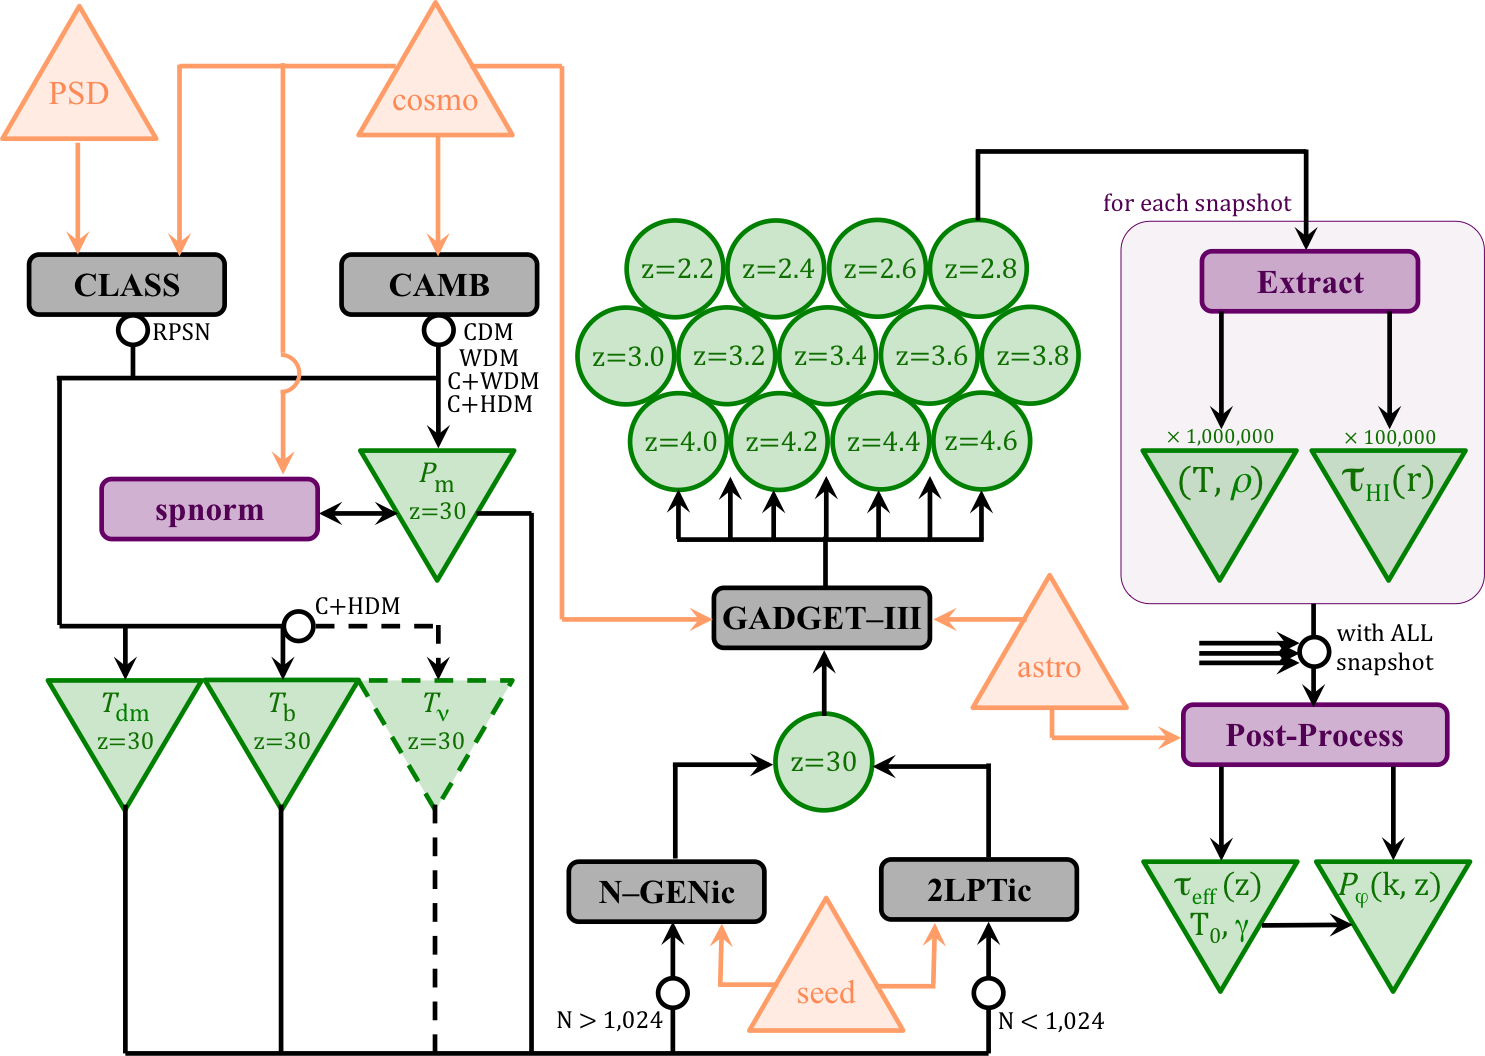
\includegraphics[width=\textwidth]{Simu/pipeline.png}
\caption{Simulation workflow. Orange triangles are user-specified inputs. Green inverted triangles are software outputs. Green circles are \texttt{Gadget} snapshot files. Black boxes are open-source codes used in our pipeline, while purple boxes are codes internal to the SDSS collaboration and python scripts generated for our specific usage. Some parts of the pipeline are only used in specific cases, specified near the small circles.}\label{fig:pipeline}
\end{figure}


A detailed assessment of our methodology is extensively provided in~\cite{Borde2014, Palanque2015a} and reviewed in~\cite{Palanque2015b}, along with all other simulation specifics including the assessment of code performance and systematics. In Fig.~\ref{fig:pipeline}, I lay out the workflow of our simulations. As mentionned in Sec.~\ref{sec:gadget}, I use the \texttt{CLASS} software for generating the matter power spectrum and transfer functions of all species at $z=30$ in the case of RPSN as cool dark matter, since it requires the particle's phase space distribution function (labelled `PSD') produced by our collaborators, Oleg Ruchayskyi, Alexei Boyarsky and Julien Lesgourgues. For all other cosmological models I investigate, be it pure WDM, C+WDM, C+HDM or any other not involving any NCDM, I use the \texttt{CAMB} software instead since the distribution functions are trivial and  are computed internally. The `cosmo' and `astro' labels refer to a set of cosmological (Sec.~\ref{sec:cosmo_param} and \ref{sec:ncdm_param}) and astrophysical parameters (Sec.~\ref{sec:astro_param}). The power spectra at $z=0$ are also generated, and the `spnorm' script re-normalizes all the power spectra and transfer functions from the specified value of $\sigma_8$, as per Eq.~\ref{eq:sig8norm} in Sec.~\ref{sec:ips}. There are $N^3$ dark matter particles treated with N-body and $N^3$ baryon particles treated with SPH, as detailed in Sec.~\ref{sec:nbody} and Sec.~\ref{sec:sph} respectively. As discussed in Sec.~\ref{sec:ips}, when involving sub-eV left-handed neutrinos as the hot component of a C+HDM cosmology, an additional $N^3$ non-interacting particles are generated with the transfer function of massive neutrinos $T_\nu (k, z=30)$ and their thermal velocities. The positions and velocities of the particles are generated with the \texttt{2LPTic} software, except if $N$ exceeds $1,024$ in which case I use the \texttt{N-GENic} software instead for ressource and memory reasons. The `seed' label refers to the integer that seeds the random drawing of the phase $\varphi$ in \ref{eq:veckphi}, and can be tweeked to generate different initial conditions, used for quantifying the sampling variance in our simulations. The result is a \texttt{Gadget} snapshot (output file) at $z=30$, which is then used to run the entire N-body + SPH section of the code described in Sec.~\ref{sec:gadget_description}, from which 13 snapshots are extracted at $\Delta z = 0.2$ steps from $z=4.6$ to $z=2.2$. The present section details the remainder of the pipeline, from which I use those \texttt{Gadget} snapshots to construct the Ly-$\alpha$ flux power spectrum.



%%%%%%%%%%%%%%%%%%%%%%%%%%%%%%
\subsection{Extracting the Power Spectrum}
%%%%%%%%%%%%%%%%%%%%%%%%%%%%%%

The \texttt{Gadget-3} snapshots contain various fields among which the position $\vec{x}$ and velocity $\vec{v}$ for dark
matter, gas particles and neutrinos if present. It also contains fields that are specific to the SPH treatment of gas particles: internal
energy $U$, density $\rho$, electron fraction ${N_e}$, hydrogen fraction $N_{\rm H}$ and the smoothing length $\ell$. I use these fields
to extract two samples: \\
\begin{itemize}
\item[$\bullet$] a subsample of particles to study the temperature-density relation. \\
\item[$\bullet$] a line of sight sample to compute the effective optical depth
\end{itemize}

\subsubsection{The IGM}
\label{sec:particle_sample}

\begin{figure}
\begin{center}
%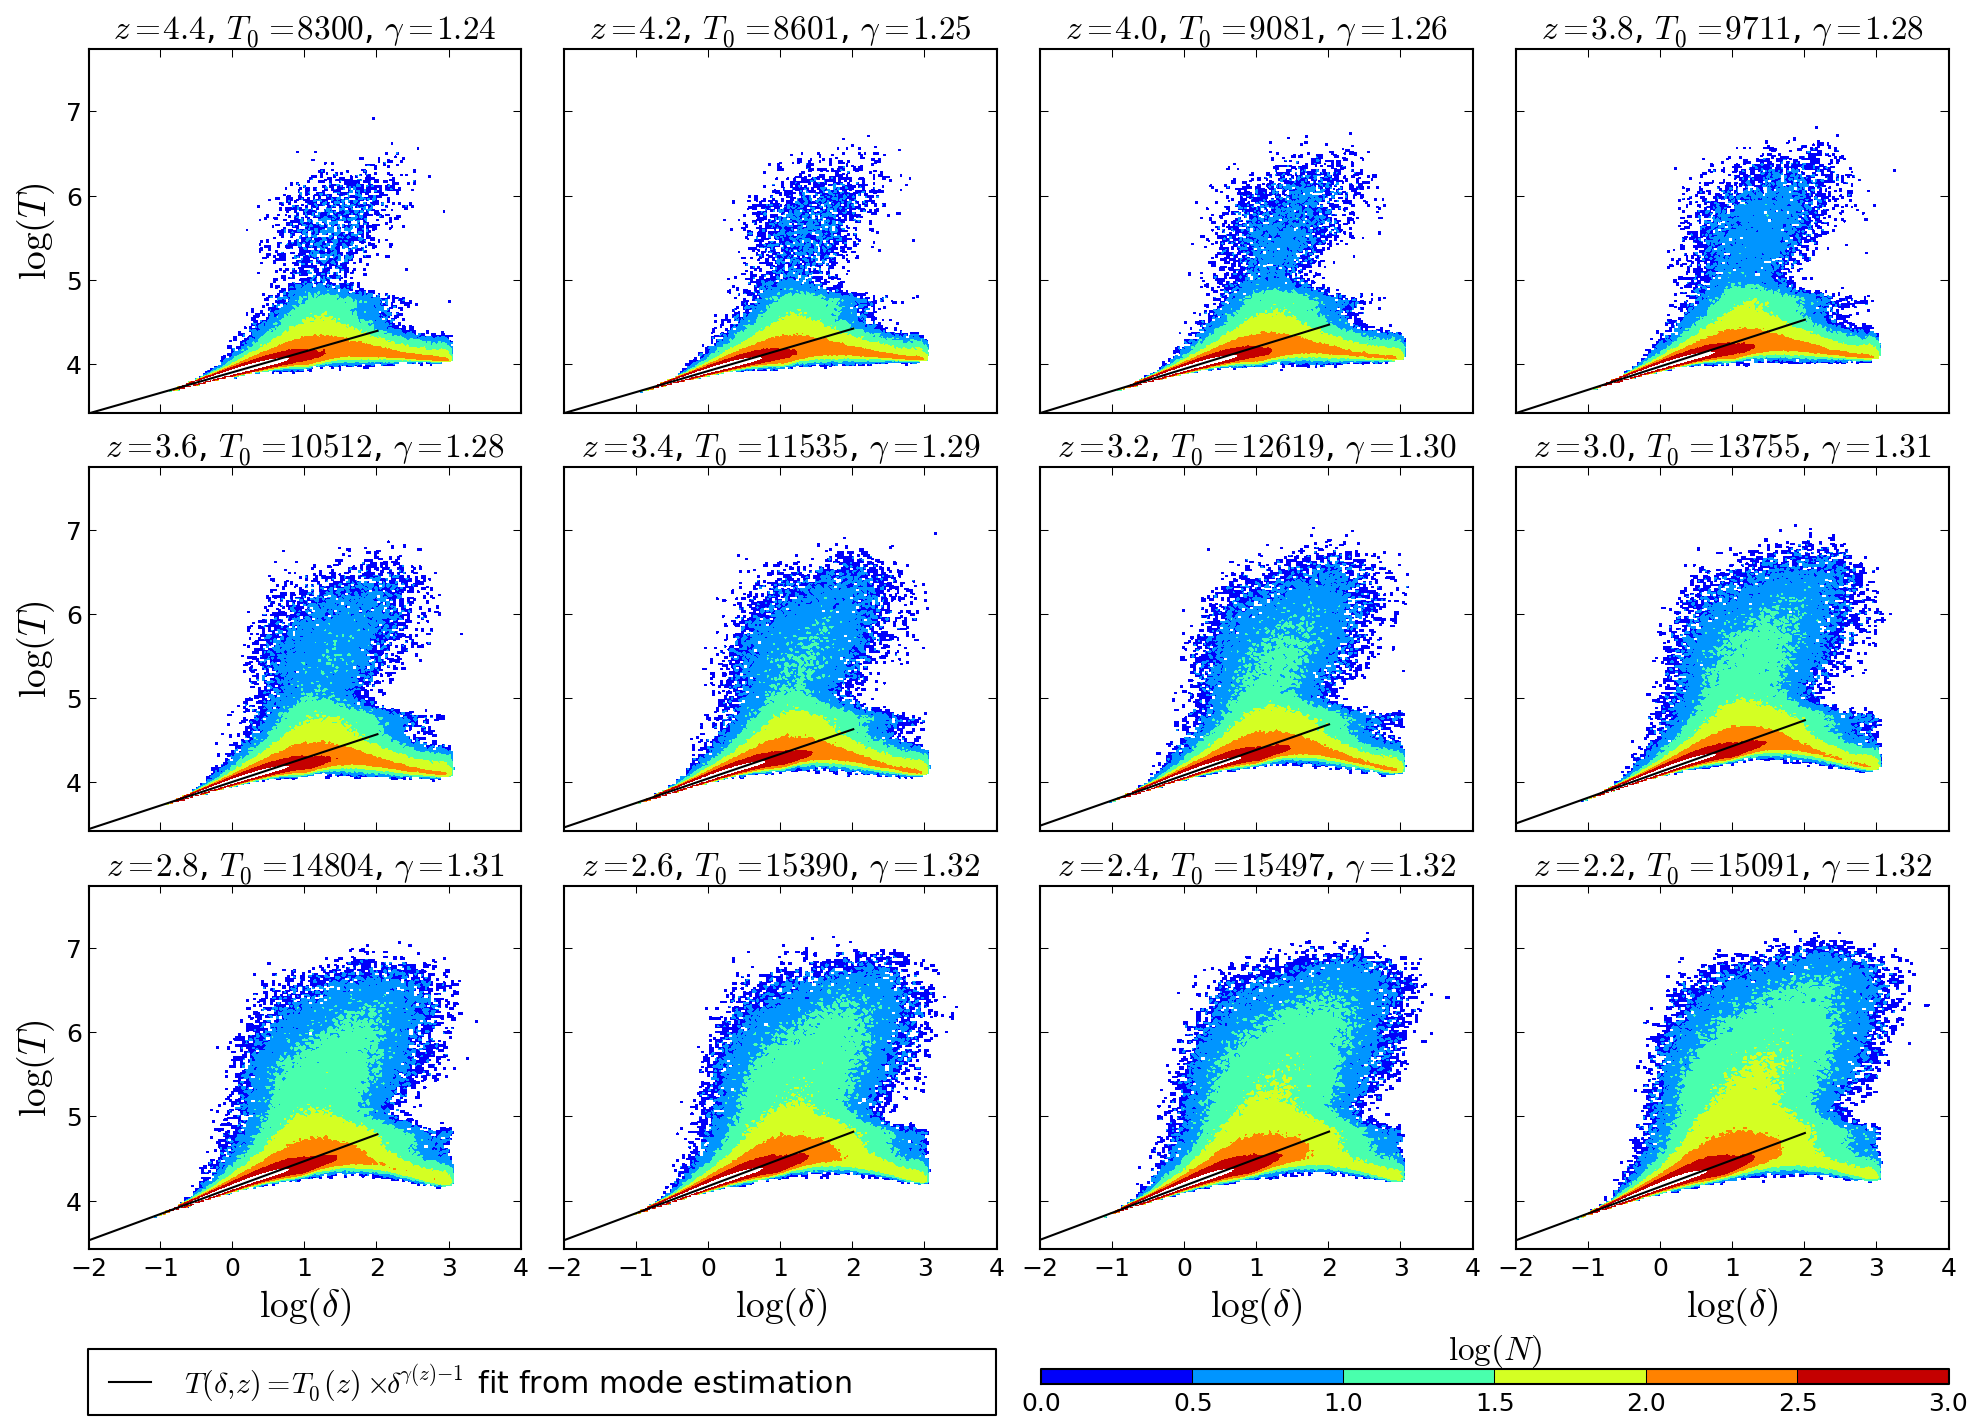
\includegraphics[width=\columnwidth]{Simu/t-rho.png}
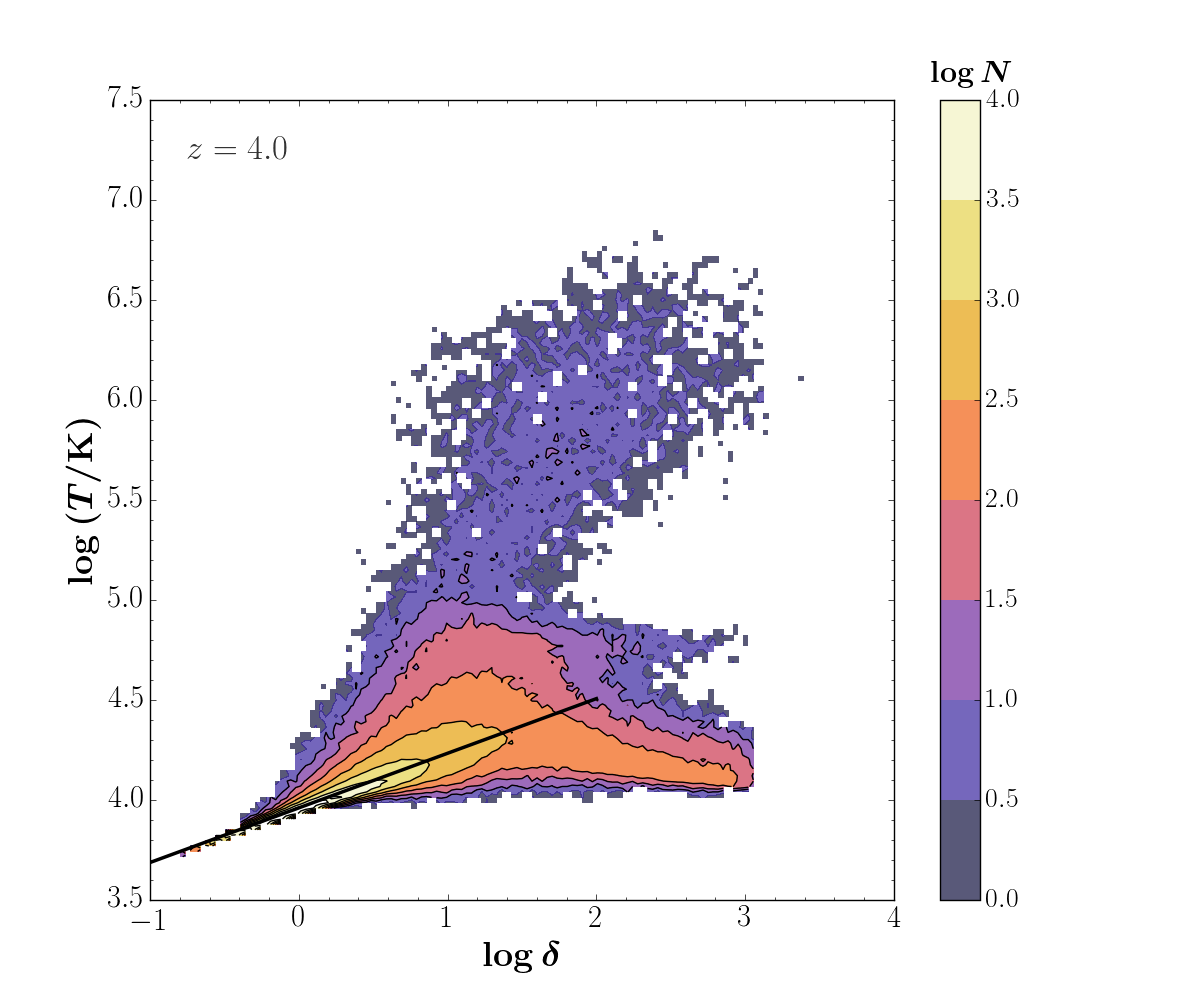
\includegraphics[width=0.5\columnwidth]{Simu/IGM_z40.png}~
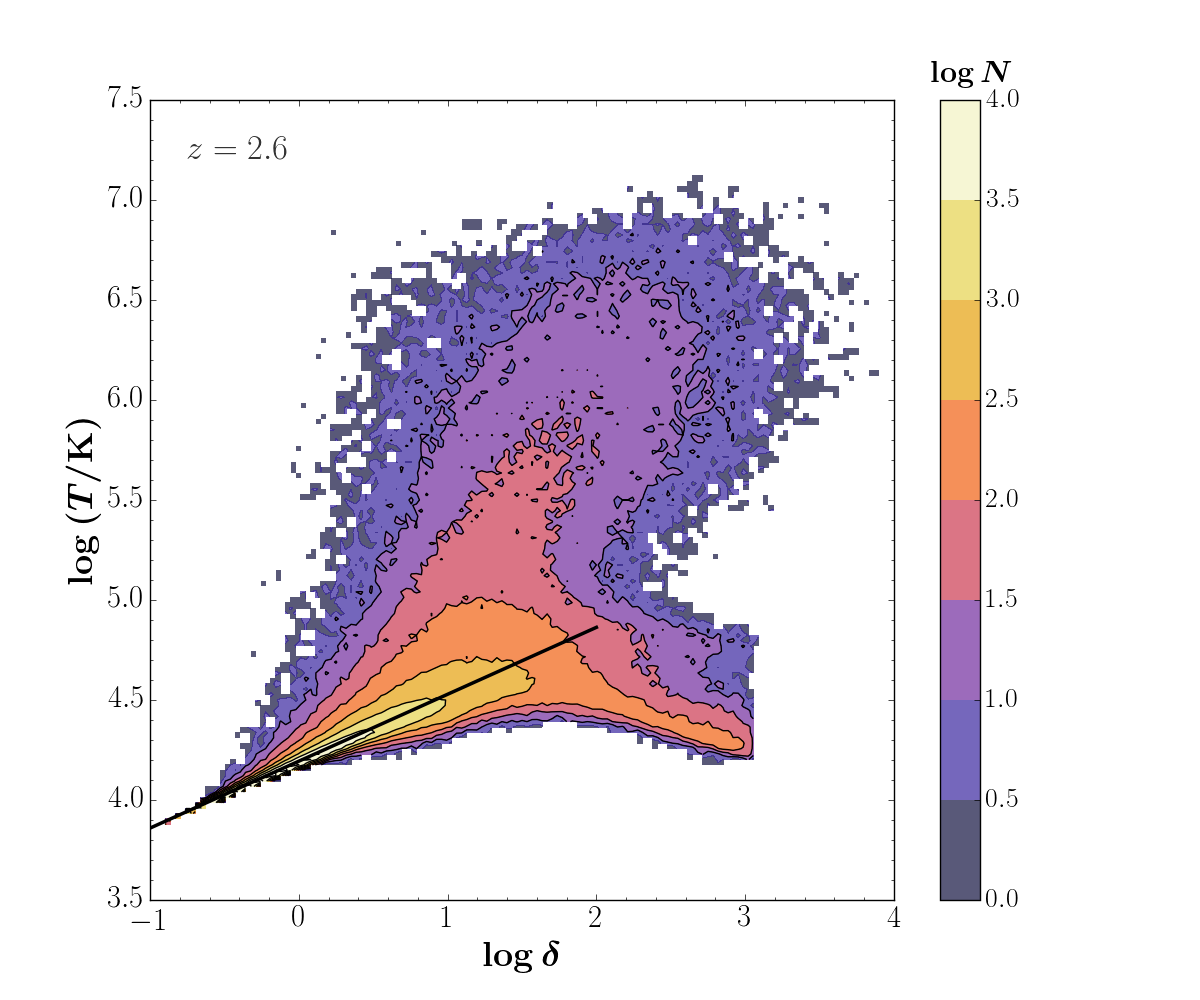
\includegraphics[width=0.5\columnwidth]{Simu/IGM_z26.png}
\caption{Temperature and density of the $10^6$ sampled particles in 2 of our 13 snapshots. The low-temperature and low-density portion of the distribution corresponds to the IGM, on which we fit the power-law amplitude and index in Eq.~\ref{eq:IGM}.}
\label{fig:rhotemp}
\end{center}
\end{figure}

For each particle the
temperature is derived with the formula 
\begin{equation}
k_b T = (\gamma -1) ~U~\times \frac{m_{\mathrm{H}}}{\frac{1}{4}+X_{\mathrm{H}} \times \left( \frac{3}{4} + N_e \right)}
\end{equation}
with $m_{\rm H}$ the mass of the Hydrogen atom and $X_{\rm H}$ the Hydrogen fraction by mass. The IGM thermal state is sparsely known at those times, and so to remain on the safe side, the IGM is treated as a monoatomic gas and the evolution its temperature as a $z$-dependant function of density is usually modeled by a simple power law
\begin{empheq}[box=\mymath]{equation}
\label{eq:IGM}
T(\rho, z) = T_0(z) \times \left( 1 + \delta \right)^{\gamma(z) - 1}
\end{empheq}

In absence of a clear consensus on the heating history of the IGM, we took the $T(\rho)$ measurements from \citet{Becker2011}
assuming $\gamma = 1.3$ as our central model, and we chose a wide variation around these values so that other recent measurements
\citep{Garzilli2012, Lidz2010, Schaye2000} fall into the explored range.
The evolution with redshift of $\gamma(z)$ and $T_0(z)$ in our simulations is therefore designed to reproduce the $T(\rho)$ measurements presented by
\citet{Becker2011} through an adaptation of the cooling routines in the simulation
code. Thus we only need to fix those two parameters at a given redshift, in our case $z=3.0$, which corresponds to the  central redshift
of our study. In practice, we do not set $T_0(z=3)$ and $\gamma (z=3)$ but instead use two internal code parameters, \texttt{AMPL} and 
\texttt{GRAD}, that alter the amplitude and  density dependence of the photo-ionization heating rates, such that
$\epsilon_f = \mathtt{AMPL} \times \delta^{\mathtt{GRAD}} \times \epsilon_i$ where the $\epsilon$'s are the heating rates and $\delta$ the
density contrast. $T_0$ and $\gamma$ are evaluated after the simulations have run, by fitting a linear regression on the low temperature and low density region of the $T-\delta$ spread in our $10^6$ particles sample, shown in Fig.~\ref{fig:rhotemp}. Given the bijective correspondence between ($T_0$, $\gamma$) and (\texttt{AMPL}, 
\texttt{GRAD}), we prefer to keep on quoting  $T_0$ and $\gamma$  since these parameters have a physical meaning and can be compared to other studies. \\

\subsubsection{The Effective Optical Depth}
\label{sec:los_sample}

The line-of-sight sample, on the other hand, uses a ray-tracing algorithm to compute the \textsc{Hi} density on $10^5$ lines-of-sight (LOS) whose origin and axis are randomly drawn, following the traditional procedure in one-dimensional flux power studies \citep{Croft2002, Gnedin2002}. For each pixel of each LOS, I derive the density
$\rho$, temperature $T$, peculiar velocity $v$ and optical depth $\tau$, all for \ion{H}{I} using the SPH equation:
\begin{equation}
A(\mathbf{r}) = \sum\limits_{i} m_i \frac{A_i}{\rho_i} W_{\mathrm{cube}} \left( \left\vert \vec{r} - \vec{r}_i \right\vert, \ell_i \right)
\end{equation} where for each particle indexed by $i$, $A$ is any of the aforementioned scalar quantities, $\vec{r}$ a position in the cube, $\ell$ the smoothing length, and $W_{\mathrm{cube}}$ the 3D cubic spline kernel introduced in Eq.~\ref{eq:cubekernel}. These LOS are not mock spectra, in the sense that they do not match any
properties (such as noise, resolution, metals absorption, \dots) of observational data. The quantity I am particularly interested in is the optical depth for \ion{H}{I}, from which I then compute the mean transmitted flux for each pixel as I describe below.\\

The extraction of these scalar quantities in each pixel of the LOS sample serves to construct the flux power spectrum, defined as the Fourier transform of the flux density contrast $\delta_\varphi = \varphi / \langle \varphi \rangle - 1$, from the effective optical depth $\tau_{\rm eff}$ where the continuum (reference) flux is defined as $\langle \varphi(z) \rangle \propto e^{- \tau_{\rm eff}(z)}$. The effective optical depth is affected mainly by the rate of ionization of Hydrogen in the IGM by stellar wind and supernovae feedbacks, as well as additional poorly-understood baryonic effects. At this stage, we fix the photo-ionization rate by rescaling the transmitted fluxes at each redshift in order to have the effective optical depth follow the empirical power-law \\
\begin{empheq}[box=\mymath]{equation} \label{eq:optdepth}
 \tau_{\rm eff}(z) = A^\tau \times \left( 1 + z \right)^{\eta^\tau}
\end{empheq} \\ When investigating the impact of the optical depth power-law index $\eta^\tau$ and amplitude $A^\tau$ in Eq.~\ref{eq:optdepth}, we do not run the \texttt{Gadget} section of the code anew, as these two astrophysical parameters are set in the post-processing part of the simulation pipeline. \\



%%%%%%%%%%%%%%%%%%%%%%%%%%%%%%
\subsection{Splicing Method}
%%%%%%%%%%%%%%%%%%%%%%%%%%%%%%

\subsubsection{Requirement}

The minimal requirements for the resolution and box size of our simulations pertain to the largest currently-available spectroscopic survey: SDSS-III/BOSS \citep{Dawson2012}. Those requirements are in part determined by the resolution of the spectrograph and the extension of the Lyman-$\alpha$ forest data (see Chapter~\ref{chap:LyaForest}). In addition, because the 1D power spectrum results from an integral over the 3D power spectrum up to $k=\infty$ (see Eq.~\ref{eq:1dps}), the resolution of the simulation has to be of the
size of the smallest structures in the transverse direction. For structures in local hydrostatic equilibrium, this would be the Jeans scale, of order $\sim 0.1~\mathrm{Mpc}$ at $z=3$. The difficulty resides in the fact that in the SPH approach, over-dense regions are sampled with a much higher spatial resolution than on average; while under-dense regions on the other hand might not necessarily be in local hydrostatic
equilibrium. A convergence test was performed to ensure that the simulations do resolve the relevant structures in \cite{Borde2014}. \\ 

The largest $k$ mode available is determined by the Nyquist-Shannon limit: $k_{\mathrm{Nyq}} = \pi / \Delta v$. The survey's constant pixel width $\Delta v = c \Delta \lambda / \lambda = 69, 20, 11~\mathrm{km}~s^{-1}$ for the SDSS pipeline \citep{Bolton2012} and the VLT's UVB and VIS arms respectively, and so $k_{\mathrm{Nyq}} = 0.045, 0.16, 0.29 ~s~\mathrm{km}^{-1}$ respectively. The spectrograph resolution requires modeling a correction factor via a window function, which preponderatly affects the largest modes. We therefore limit our analysis to $k_{\mathrm{Nyq}}/4$. \\

The smallest $k$ mode we can probe is set by the portion of the Ly-$\alpha$ forest that extends between the Ly-$\alpha~\lambda1216$ and Ly-$\beta~\lambda1026$ emission lines. The exploitable Ly-$\alpha$ forest is actually smaller than the separation of those two emissions due to their respective widths. In addition, instrumental constraints often make the first and last theoretical modes very difficult to obtain with reasonable precision from data. \citet{McDonald2006} used the $1041 < \lambda_0/\AA < 1185$ region, which corresponds to $\Delta v \simeq 4 \times 10^4~\mathrm{km}~s^{-1}$ and $k_{\mathrm{min}} = 1.6 \times 10^{-4} s~\mathrm{km}^{-1}$. However, they restricted their analysis to $k_{\mathrm{min}} = 1.4 \times 10^{-3} s~\mathrm{km}^{-1}$ and $k_{\mathrm{max}} = 1.8 \times 10^{-2} s~\mathrm{km}^{-1}$. Using the most recent Ly-$\alpha$ BOSS data from DR9, the 1D power spectrum was computed from forest lengths corresponding to a third of the total available range. This enabled restraining the redshift span to at most $\Delta z=0.2$ (see Chapter~\ref{chap:LyaForest}). As a consequence,  the lowest mode is set to $k_{\mathrm{min}} \simeq 1.0 \times 10^{-3} s~\mathrm{km}^{-1}$. \\

In summary, when using BOSS data, we consider simulations that cover the range $10^{-3} \leqslant k / (\mathrm{km}/s)^{-1} \leqslant 2 \times 10^{-2}$, corresponding to $0.1 \leqslant k / (\mathrm{Mpc}/h)^{-1} \leqslant 2$ at $z \simeq 3$. When using XQ-100 data, we can extend the maximum mode to $5-7~\times 10^{-2}~s~\mathrm{km}^{-1}$, depending on the redshift (see upper panel of Fig.~\ref{fig:hr_mr}). The high resolution of the MIKE and HIRES data sets make it possible to exploit a $k_{\mathrm{max}} = 8 \times 10^{-2} ~s~\mathrm{km}^{-1}$ point. In anticipation of future surveys, I've adapted the pipeline to compute the flux power spectrum in the range $10^{-3} \leqslant k / (\mathrm{km}/s)^{-1} \leqslant 10^{-1}$, corresponding to $0.1 \leqslant k / (\mathrm{Mpc}/h)^{-1} \leqslant 10$ at $z \simeq 3$. \\

On the numerical simulations side, the two relevant parameters that determine the available $k$ range are the length of the box $L$ which determines the smallest exploitable $k$; and the $N/L$ ratio (which can be interpreted as the resolution cube-rooted) which determines the largest exploitable mode. It is worthy to note that in currently used algorithms such as SPH or Adaptive Mesh Refinement (AMR) in which the resolution emulates the density, so-to-speak, particle spacing in regions of interest will be significantly smaller
than $L/N$. However, to remain on the safe conservative side, I still limit the maximum mode to this approximation. When evolving $N^3$ particles in a box of volume $L^3$, our available range of exploitable modes is thus
\begin{equation}
\frac{2 \pi}{L} = k_{\mathrm{min}} \leqslant k \leqslant \frac{k_{\mathrm{Nyq}}}{4} = \frac{1}{4} \frac{2 \pi N}{2 L}
\end{equation}

\begin{figure}
\begin{center}
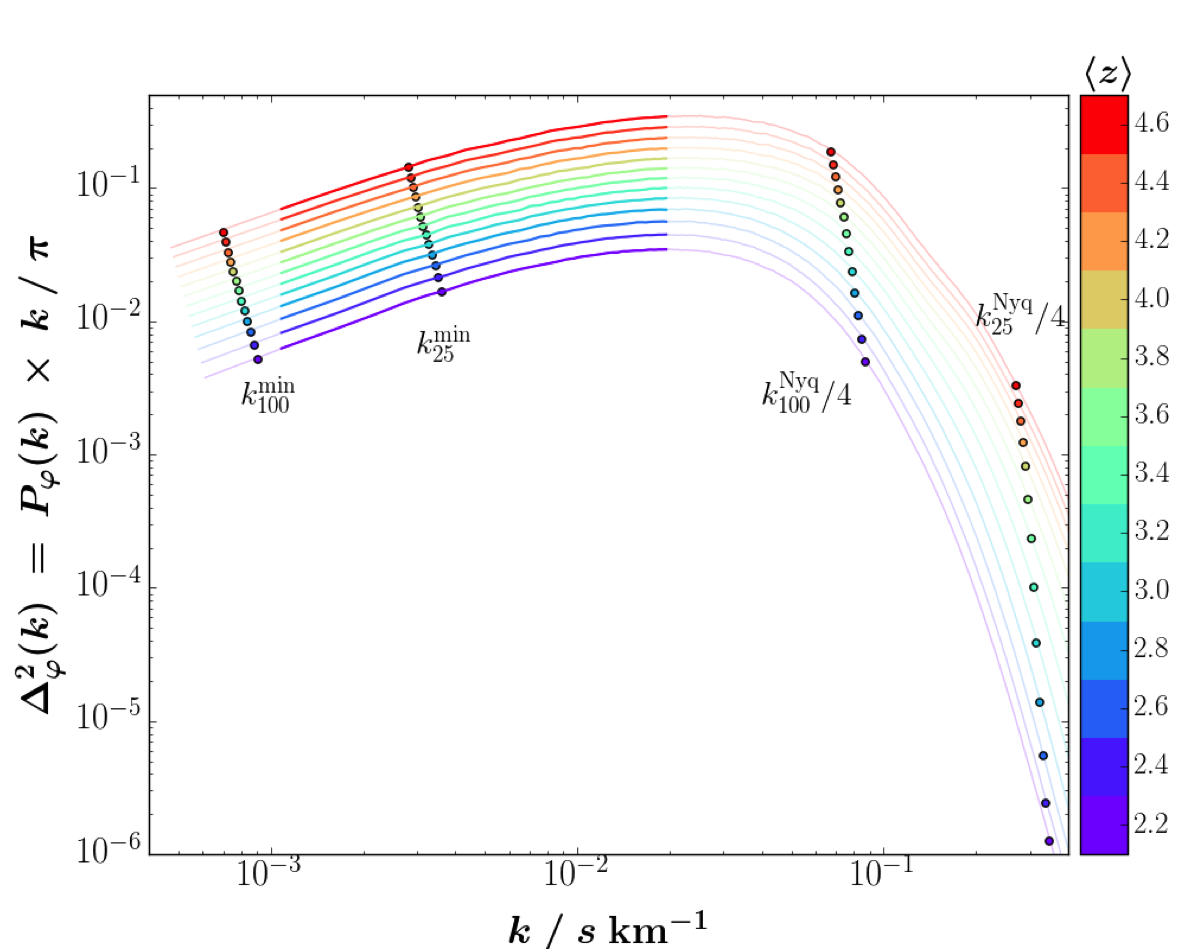
\includegraphics[width=0.75\columnwidth]{highresopfluxsimu.png}
\caption{Dimensionless flux power spectrum of the benchmark CDM model, from redshift $z=2.2$ to $4.6$ (color coded). The $L=100 ~(25) ~h^{-1}\mathrm{Mpc}$ simulations are relevant only in the $ \left( k^{\mathrm{min}}_{100 (25)}, k^{\mathrm{Nyq}}_{100 (25)} / 4 \right)$ range respectively, which overlap in the central region. The highlighted segments are the modes in the BOSS DR9 Ly-$\alpha$ forest power spectrum range.}
\label{fig:hrpsimu}
\end{center}
\end{figure}

Therefore, the theoretical minimum requirement for a simulation to reproduce the BOSS DR9 data precision is a box of about $100~h^{-1} \mathrm{Mpc}$ with $\sim 100^3$ particles of each type. Convergence tests were performed in \cite{Borde2014} to refine these requirements. In particular, they showed that many more particles were needed to achieve the required resolution, to the tail end of $N=3072$.
Fig.~\ref{fig:hrpsimu} displays the flux power spectra of a generic simulation (in the \emph{best guess} configuration) in all 13 redshift bins. I've pinpointed the minimum and maximum $k$ modes that bound our analysis for the $L=25~h^{-1}\mathrm{Mpc}$ and $L=100~h^{-1}\mathrm{Mpc}$ box sizes as a function of redshift. The highlighted region is where we interpolate the power spectrum in the adequate array of $k$ values to compare to SDSS/BOSS data.

\subsubsection{Splicing Principle}

A $(L/h^{-1}\mathrm{Mpc}, N) = (100, 3072)$ hydrodynamics simulation is computationally expensive to run on a tier-1 supercluster like \texttt{Curie}, \texttt{MareNostrum}, \texttt{Hazel Han}, \textit{etc}. The many simulations required to perform our analysis (of the order $10^{1-2}$) would be inefficient to the point of impractical. To circumvent this resource and time dilemna, I make use of a \emph{splicing} technique described in~\cite{McDonald2003} and first applied in~\cite{Borde2014,Palanque2015a}. I use it to infer the flux power spectrum of the equivalent to a $(100, 3072)$ simulation from a combination of three lesser ones: a scaled-down $(25, 768)$ to provide high resolution on small scales (labelled \textbf{HR} for `high resolution'), a large-box low-resolution $(100, 768)$ for large scales (labelled \textbf{HL} for `high $L$'), and a small-box low-resolution $(25, 192)$ to bridge the preceding two at intermediate scales (labelled \textbf{TR} for `transition'). In addition to saving considerable time and resource consumption, this splicing technique loopholes around the limits of the software and packages we utilize in our pipeline. \\

\begin{figure}
\begin{center}
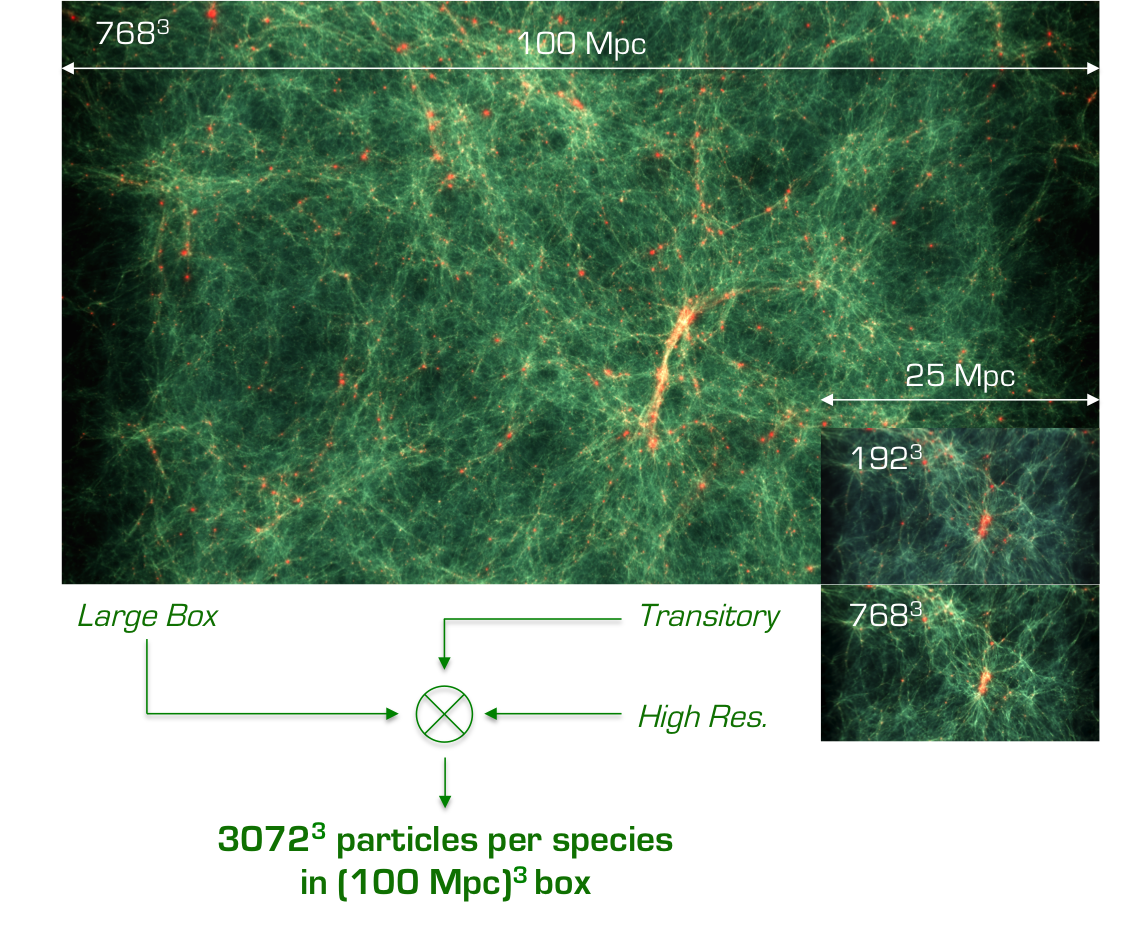
\includegraphics[width=0.75\columnwidth]{Splicing/splicingprinciple.png}
\caption{Schematic of the 3 simulations used in the splicing method, rendered with the \texttt{Sploth} software. }
\label{fig:splicingprinciple}
\end{center}
\end{figure}

While a $(100, 3072)$ hydrodynamics simulation would require $\sim 5 \times 10^6$ CPU hours, the HL-HR-TR trio set only consumes $\sim 10^5$ CPU hours in total. The bridging of these 3 power spectra into their equivalent power spectrum is illustrated in Fig.~\ref{fig:splicingprinciple} and goes as follows. Let us adopt a more general notation and write the HL-HR-TR set as $(L, N)$, $(L/4, N)$ and $(L/4, N/4)$, which is used to infer the power spectrum of an equivalent $(L, 4N)$ simulation. Notice the HR simulation has the correct resolution but lacks in volume by a factor $4^3 = 64$. The idea is to correct for its small size with the help of the HL simulation, which has the correct size but lacks in resolution by that same $4^3=64$ factor. To perform the bridging, we make use of the TR simulation which has the same resolution as HL while having the same volume as the HR. As visible in Fig.~\ref{fig:hrpsimu}, the minimum and maximum modes for the small and large box size simulations distinguish between 3 regimes:\\
\begin{itemize}
\item[$\bullet$] Below $k \leqslant k_{L/4}^{\mathrm{min}}$, only HL is relevant. Consequently, we have no choice but to set the finalized power spectrum of the $(L, 4N)$ to that of the $(L, N)$ simulation and correct for its low resolution by a $k$-independant factor evaluated at $k_{L/4}^{\mathrm{min}}$:
	\begin{equation}
	\label{eq:low_regime}
	P_{\varphi}^{(L, 4N)} (k \leqslant k_{L/4}^{\mathrm{min}}) = P_{\varphi}^{(L, N)} (k \leqslant k_{L/4}^{\mathrm{min}}) ~\times~ \left. \frac{P_{\varphi}^{(L/4, N)}}{P_{\varphi}^{(L/4, N/4)}} \right\vert_{k=k_{L/4}^{\mathrm{min}}}
	\end{equation}
where the dependance on $z$ is implicit in all quantities, including $k_{L/4}^{\mathrm{min}}(z)$. \\
\\
\item[$\bullet$] Above $k \geqslant k_{L}^{\mathrm{Nyq}}/4$, only HR is relevant. Similarly, we have no choice but to set the finalized power spectrum of the $(L, 4N)$ to that of the $(L/4, N)$ simulation and correct for its small size by a $k$-independant factor evaluated at $k_{L}^{\mathrm{Nyq}}/4$:
	\begin{equation}
	\label{eq:intermediate_regime}
	P_{\varphi}^{(L, 4N)} (k \geqslant k_{L}^{\mathrm{Nyq}}/4) = P_{\varphi}^{(L/4, N)} (k \geqslant k_{L}^{\mathrm{Nyq}}/4) ~\times~ \left. \frac{P_{\varphi}^{(L, N/4)}}{P_{\varphi}^{(L/4, N/4)}} \right\vert_{k=\geqslant k_{L}^{\mathrm{Nyq}}/4}
	\end{equation} \\
\\
\item[$\bullet$] In the intermediate range, $k_{L/4}^{\mathrm{min}} \leqslant k \leqslant k_{L}^{\mathrm{Nyq}}/4$, both HL and HR can be exploited. This time, the correction factor is $k$-dependant and
	\begin{equation}
	P_{\varphi}^{(L, 4N)} (k_{L/4}^{\mathrm{min}} \leqslant k \leqslant k_{L}^{\mathrm{Nyq}}/4) = P_{\varphi}^{(L/4, N)} (k) ~\times~  \frac{P_{\varphi}^{(L/4, N)}(k)}{P_{\varphi}^{(L/4, N/4)}(k)}
	\end{equation} \\
\end{itemize}

Tab.~\ref{tab:splice_params} explicits the values of $(L/h^{-1}\mathrm{Mpc}, N)$ for each of the spliced set of simulations destined to model their corresponding 'exact' simulation.


\subsubsection{Residuals}


\begin{table}
	\begin{center}
	\begin{small}
		\begin{tabular}{ccccc}
			\textbf{exact run} &  \multicolumn{3}{c}{\textbf{splicing trio}} & \textbf{residual average}\\[2pt]
			\hline \\[-10pt]
			 & \textbf{HL} & \textbf{HR} & \textbf{TR} & \\[2pt]
			$\pmb{\left( L, N \right)}$ & $\pmb{\left( L, N/4 \right)}$ & $\pmb{\left( L/4, N/4 \right)}$ & $\pmb{\left( L/4, N/16 \right)}$ & $\Delta P(k,z) / P(k,z)$ \\[2pt]
			\hline \\[-10pt]
			\\[-10pt]
			$(100, 1600)$ & $(100, 400)$ & $(25, 400)$ & $(25, 100)$ & $\sim 3 \%$ \\[2pt]						
			$(100, 1024)$ & $(100, 256)$ & $(25, 256)$ & $(25, 64)$ & $\sim 3 \%$ \\[2pt]						
			$(100, 2046)$ & $(100, 512)$ & $(25, 512)$ & $(25, 128)$ & $\sim 2 \%$ \\[2pt]						
			$(100, 3072)$ & $(100, 768)$ & $(25, 768)$ & $(25, 192)$ &  \\[2pt]						
			\hline \\[-10pt]
		\end{tabular}
	\end{small}
	\end{center}
	\caption{First column: `exact' simulation. Second, third and fourth columns: `HL', `HR' and `TR' splicing trio corresponding to the exact run it emulates. Last column gives the average value of the residual averaged over $k$ and $z$. Note the (100, 3072) simulation has never been run, and so the splicing residual is extrapolated from the lower resolution simulations.}
	\label{tab:splice_params}
\end{table}


This procedure introduces an additional simulation uncertainty, which is encoded in the residual between the spliced power spectrum with respect to the exact power spectrum $r(k, z) = \Delta_\varphi P(k, z) / P_\varphi(k, z)$. I've managed to adapt the pipeline to successfully run the `exact' simulations for $N=1024, 1600$ and $2048$, which required switching from \texttt{2LPTic} to the \texttt{NGENic} software, parallelizing the \texttt{Gadget} code on $\sim 8,000$ of the \texttt{Curie} machine's thin nodes and all the associated ressource/memory careful re-allocation, producing the output files in $256$ seperate files and adapting the \texttt{Extract} code to read and write from each of these files on \texttt{Curie}'s extra-large nodes. At the time I ran the $(100, 2048)$ simulation, which consumed approximately $\sim 5 \times 10^5$ CPU hours, it was the largest and most resolute simulation of its kind (using SPH). Not only did it require 2 failed attempts before succeeding, but our ressource allocation by \texttt{PRACE} restricted us to only exploit 5 redshift snapshots: $z=2.2, 3.0, 3.4, 4.0$ and $4.4$. Fig.~\ref{fig:residual_and_zoom} displays the splicing residual for three of these redshifts. The $N=1024$ and $N=1600$ runs were useful not only in characterizing the $k$ and $z$ dependance of the splicing residuals at these resolutions, but definitely served as useful and insightful preliminary practice, during which many computational ressources were spent, but many valuable lessons were learned. \\


\begin{figure}
\begin{center}
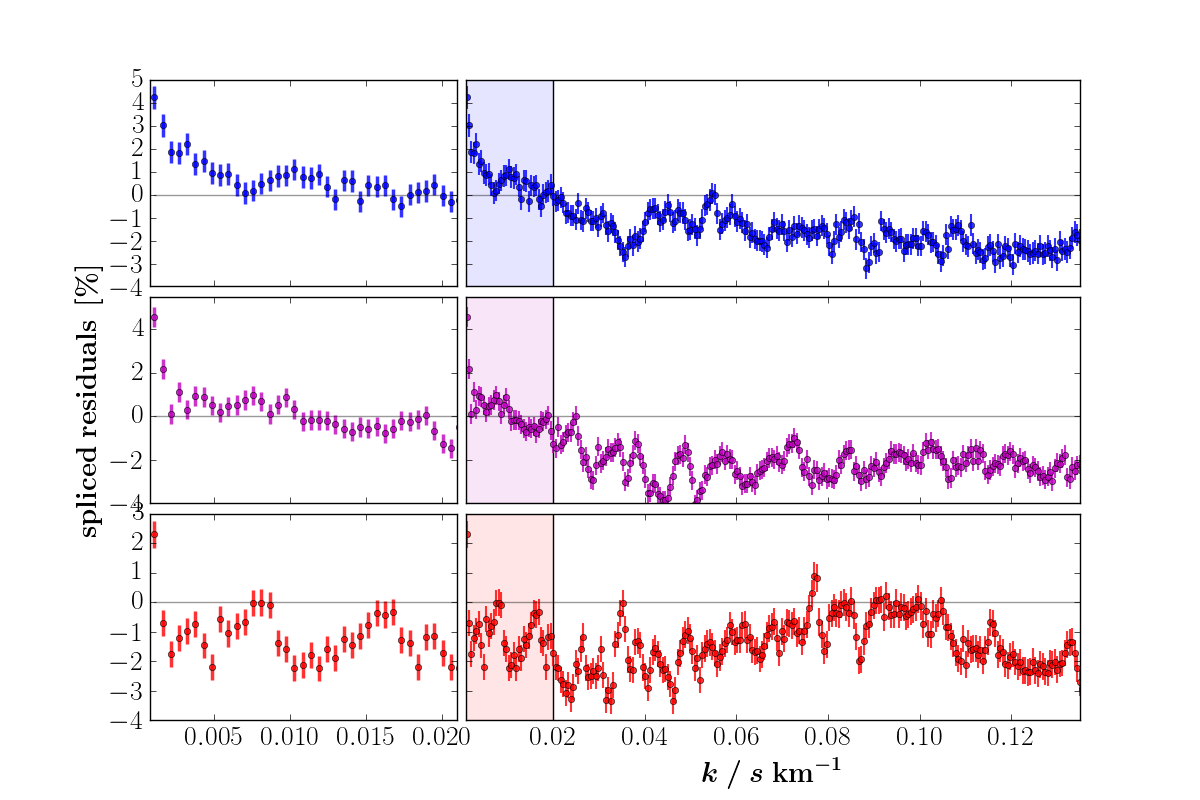
\includegraphics[width=\columnwidth]{Splicing/Splicing_2048.png}
\caption{Splicing residuals for the $N=2048$ run at $z=2.2$ (top, blue), $z=3.4$ (middle, purple) and $z=4.4$ (bottom, red). Left-hand panels are zooms on the highlighted regions, which is the range relevant for BOSS. The error bars correspond to simulation shot noise.}
\label{fig:residual_and_zoom}
\end{center}
\end{figure}

The splicing residuals are modeled by lines in all three sectors defined in the previous subsection. Since all of our data sets fall below the $k_{100}^{\mathrm{Nyq}}/4 \sim 0.1~s/\mathrm{km}$, we only fit our line parameters in the two lower regimes, distinguished from one another by the pivot scale $k_{L/4}^{\mathrm{min}}(z)$. In the intermediate regime, where the splicing correction factor is $k$-dependant, the residuals are modeled by a flat line (zero slope), which is expected since the $k$-dependance appears in both the numerator and denominator of Eq.~\ref{eq:intermediate_regime}, and so the residuals between the HL and exact simulations are expected to be simply offset by a quasi-constant factor. In the large-scale portion (low $k$), \textit{i.e.} below the pivot scale, the residuals follow a steeply declining line whose slope flattens with redshift, which here again is expected from the expression in Eq.~\ref{eq:low_regime}. Since the intermediate regime offset and the lower regime line intersect at the pivot scale, which is fixed, we only require 2 degrees of freedom to characterize the residuals: the slope $dr/dk$ and the offset $r(k_p, z)$: \\
\begin{equation}
\label{eq:splicing_dof}
\left\{
\begin{array}{l}
r(k \leqslant k_p, z) = \cfrac{d r}{d k} (z) \times (k-k_p) + r(k_p, z) \\
\\
r(k \geqslant k_p, z) = r(k_p, z)
\end{array}
\right.
\end{equation} \\ where $k_p = k_{25}^{\mathrm{min}}$ is the ($z$-dependant) pivot scale. This model is an improvement upon the one used previously, where the accuracy of the splicing technique was estimated from less resolved simulations and modeled by a single redshift-independent linear function of $k$ over all modes. Our working group applied this new model of the splicing residuals to the work published in \cite{Palanque2015b}, and all subsequent works, \textit{e.g.} \cite{Baur16, Yeche17, Armengaud_FDM, Baur17}.


%%%%%%%%%%%%%%%%%%%%%%%%%%%%%%
%\subsection{Visual Inspection}
%%%%%%%%%%%%%%%%%%%%%%%%%%%%%%

%\subsubsection{The Transfer Equation}

%\begin{equation}
%\rho (\vec{r}) \frac{\partial I(\vec{r})}{\partial r} + A I(\vec{r}) - E = 0
%\end{equation}

%\subsubsection{The \textsf{Splotch} Software}

%\begin{figure}
%\begin{center}
%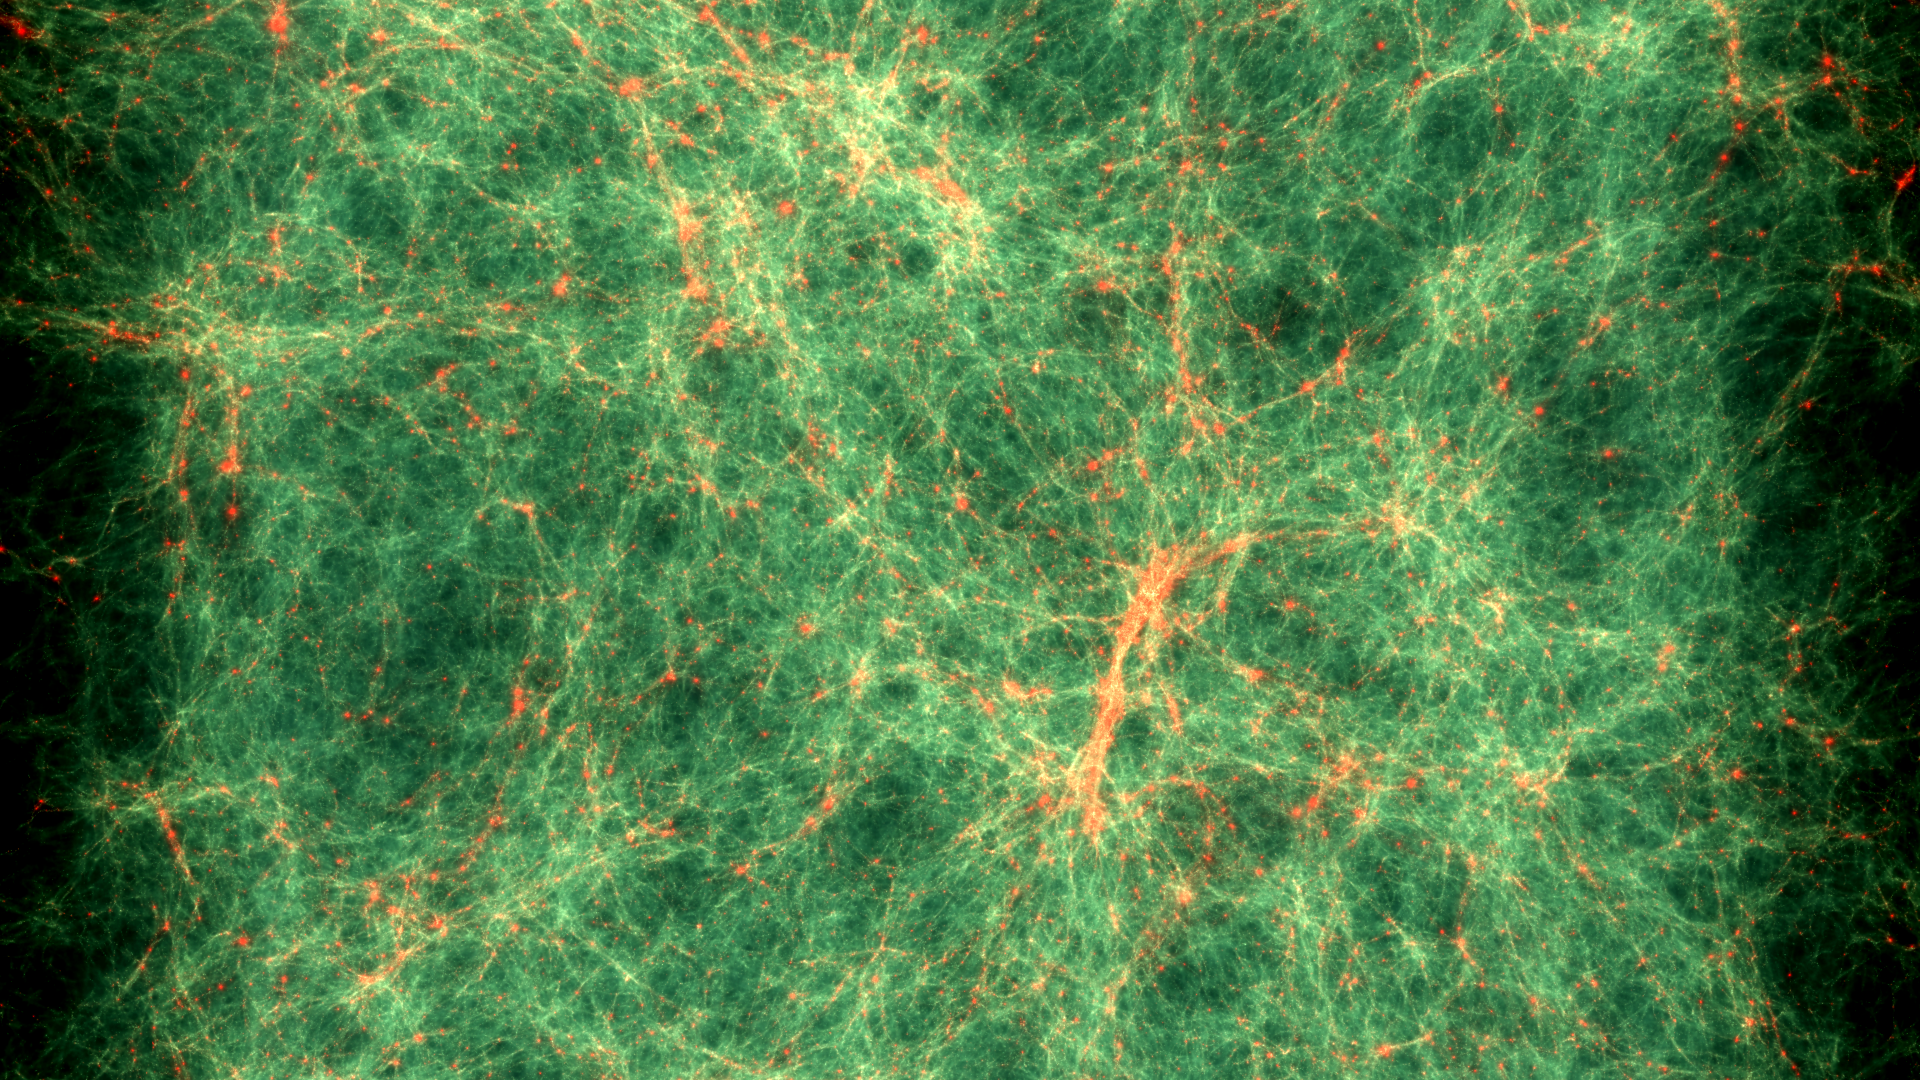
\includegraphics[width=0.9\columnwidth]{Visu/CDM_z22.png}
%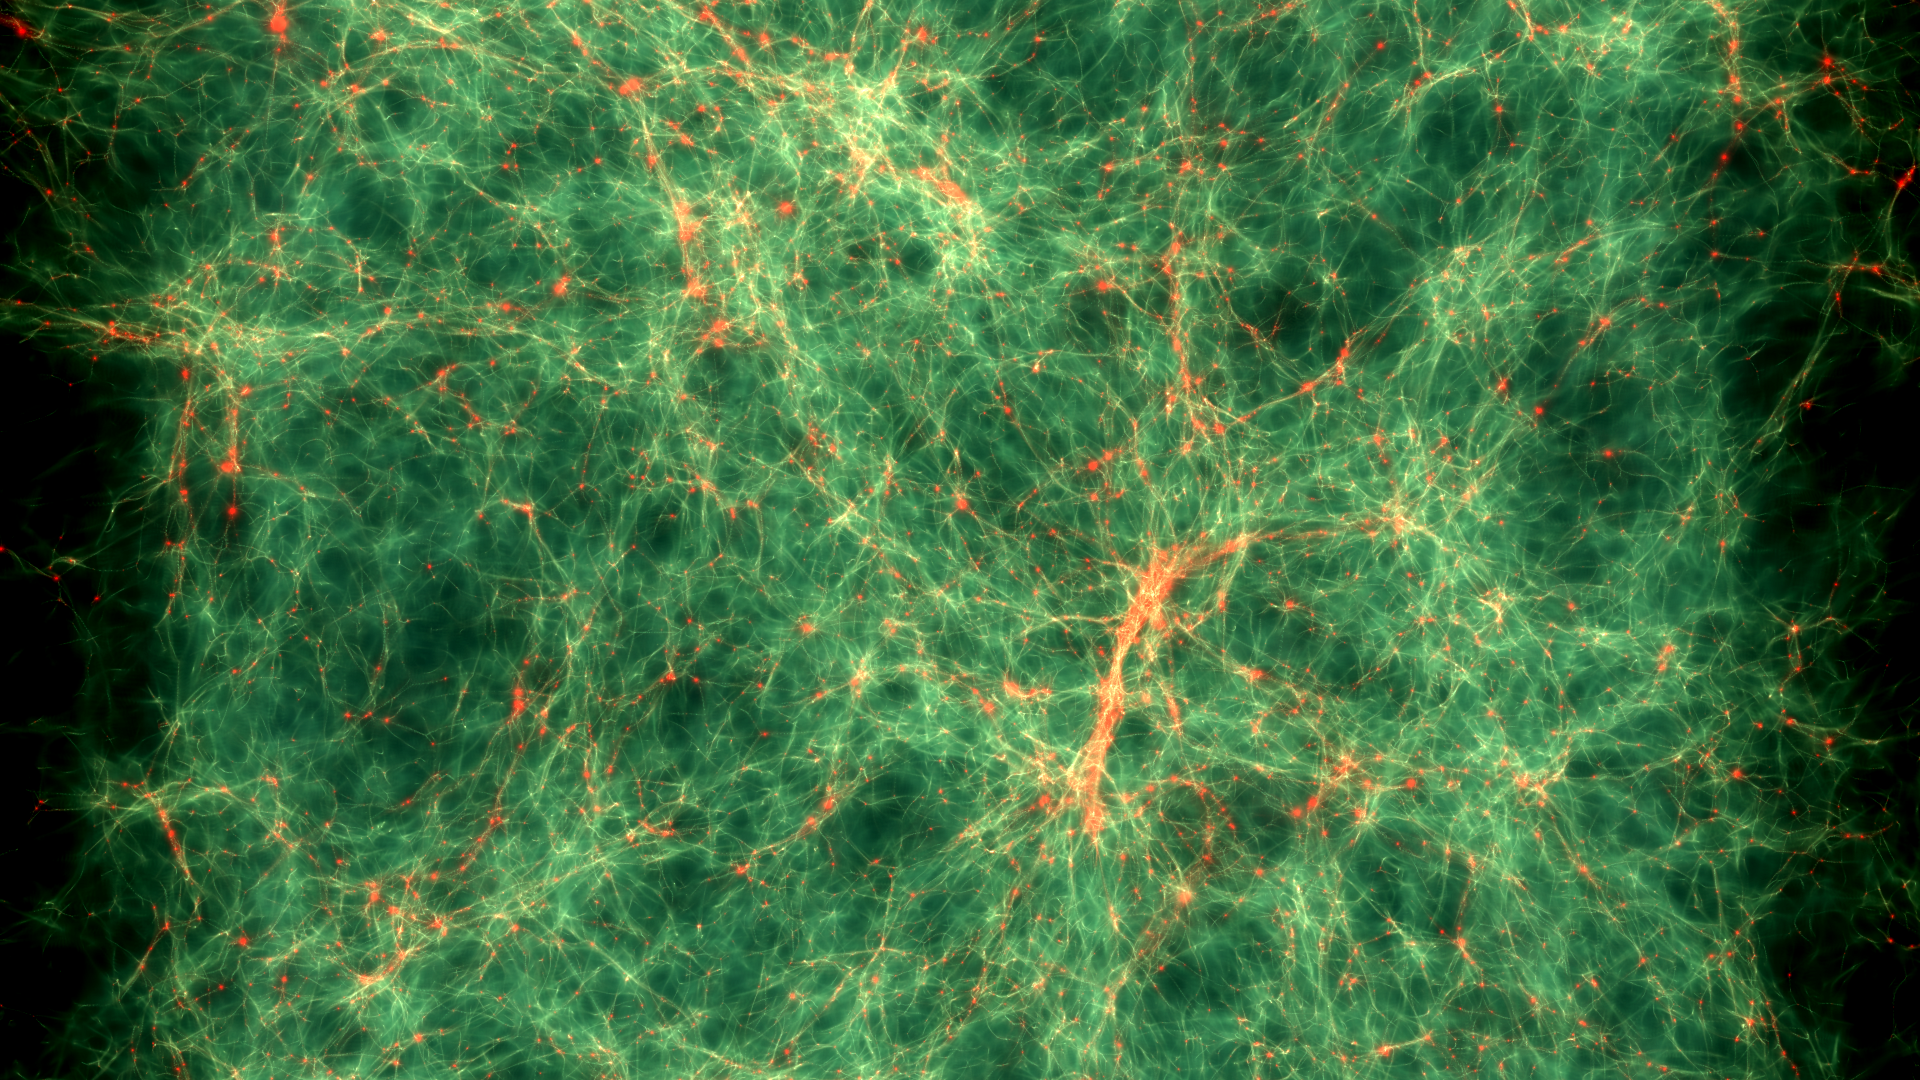
\includegraphics[width=0.9\columnwidth]{Visu/HDM_500eV_z22.png}
%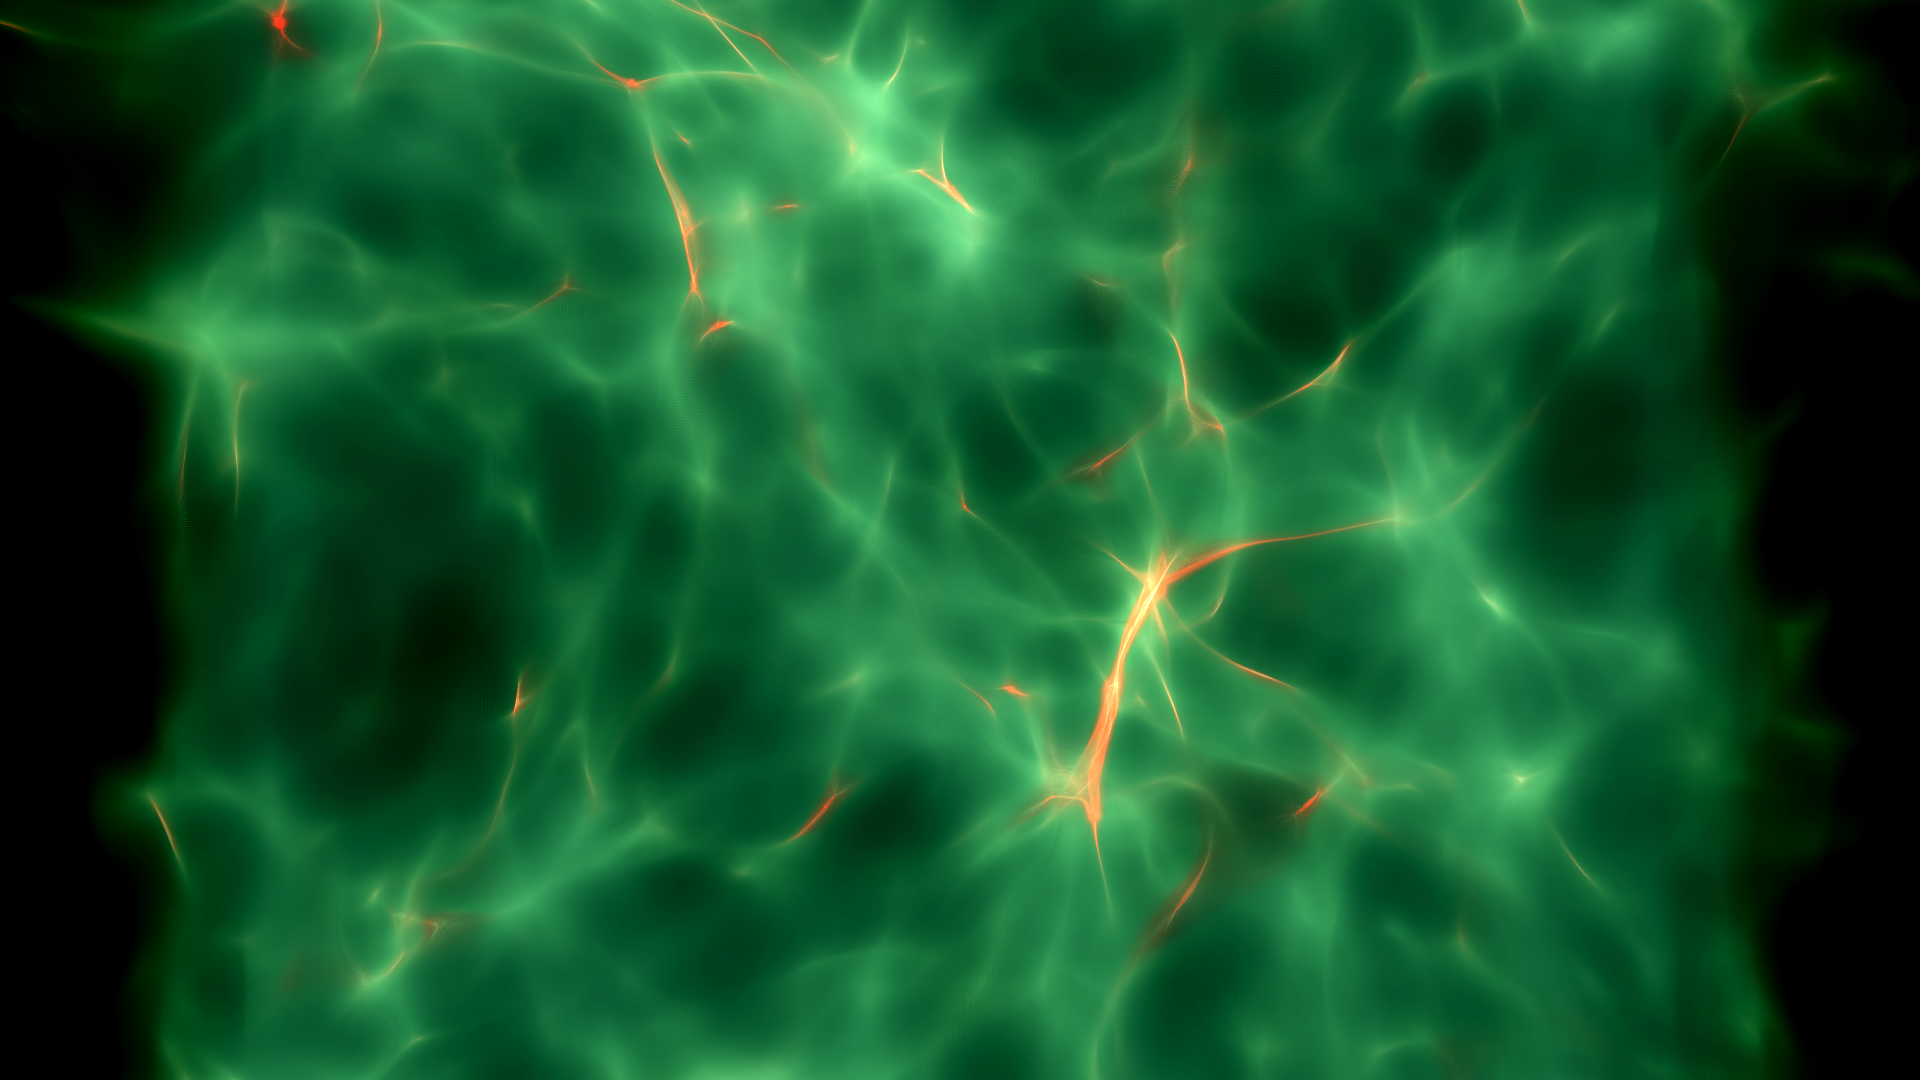
\includegraphics[width=0.9\columnwidth]{Visu/HDM_100eV_z22.png}
%\caption{.}
%\end{center}
%\label{fig:visu_splotch}
%\end{figure}


\begin{figure}
\begin{center}
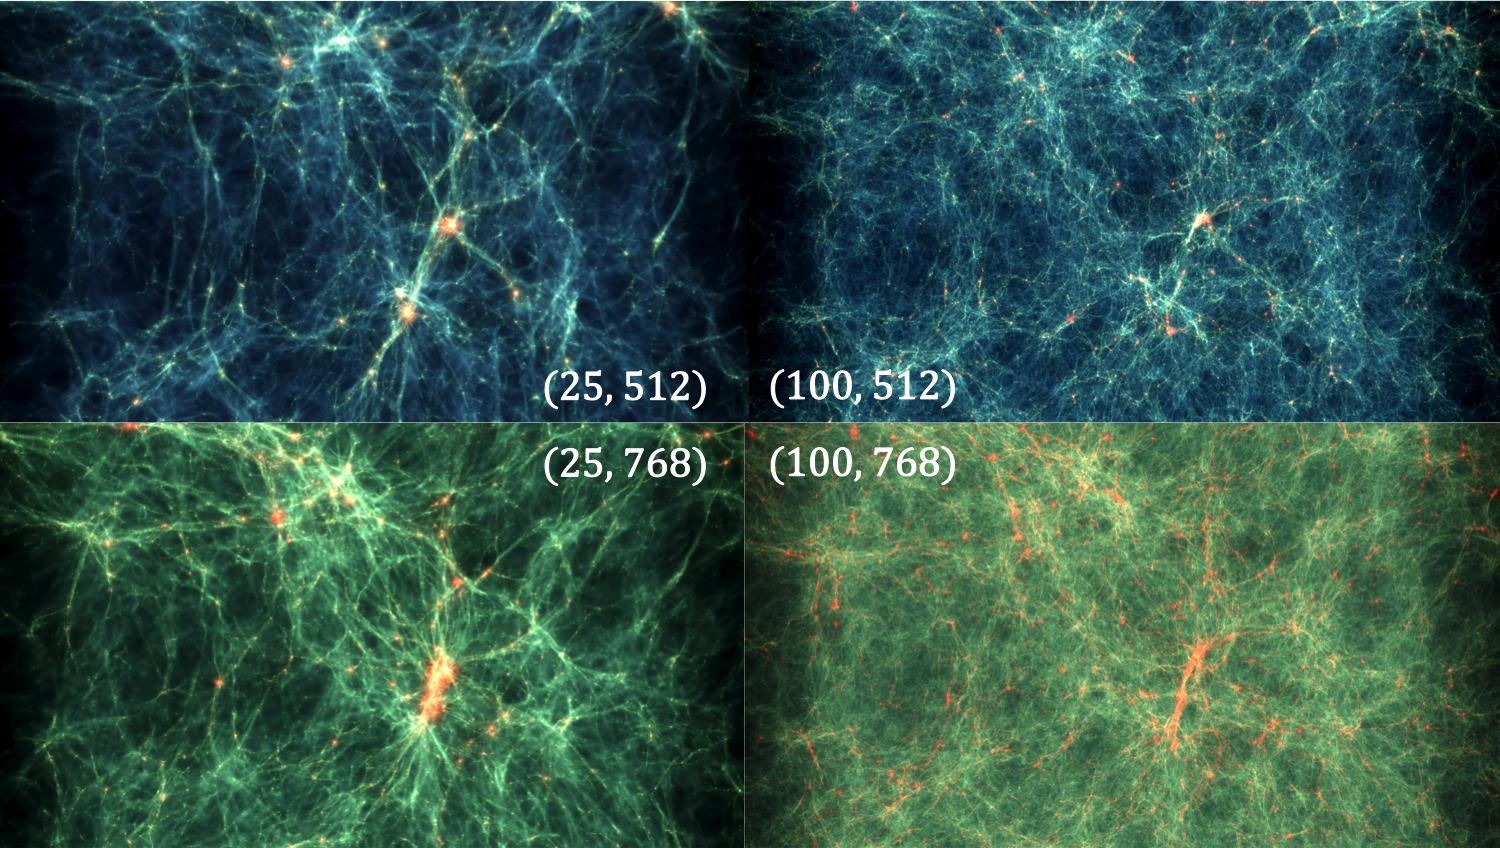
\includegraphics[width=\columnwidth]{Visu/HRHL.png}
\caption{HR (left) and HL (right) simulations used to splice the power spectrum into the equivalent of an $N=2048$ (top) and $N=3072$ (bottom) resolution. Baryon temperature and density is rendered by the \texttt{Splotch} software. Note the stark difference in contrast from one resolution to the other, despite all having the same seed.}
\end{center}
\label{fig:visu_splice}
\end{figure}

\clearpage